\section{Propagation of the Particles and Light}
\label{sec:propagation}
\subsection{Modeling with GEANT4}
\label{subsec:geant}
I don't know shit about geant4.
Something about how great and wonderous and slow it is at doing particle interactions at low energy.

\subsection{Lepton Propagation with PROPOSAL}
\label{subsec:proposal}

\begin{figure}
\centering
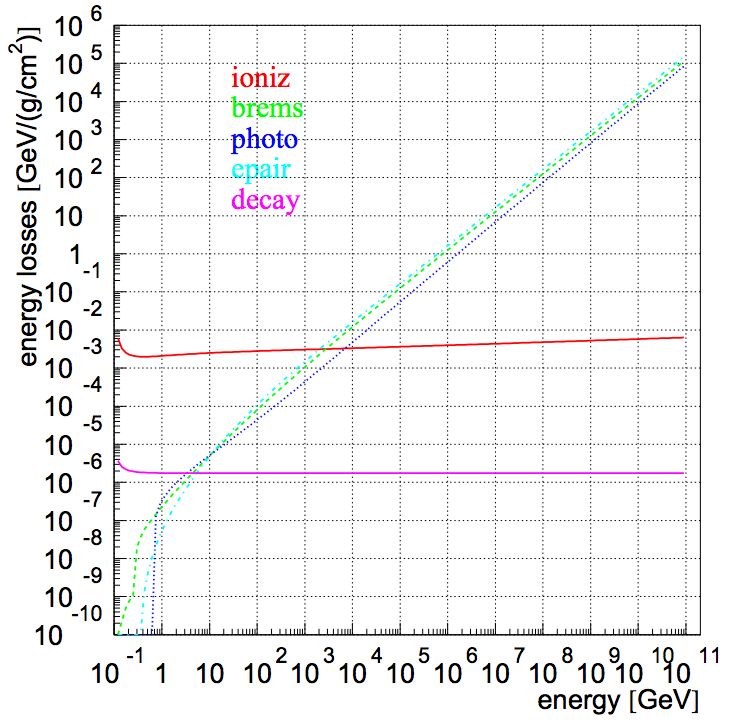
\includegraphics[width=0.6\linewidth]{discrete_emissions_MMC.png}
\caption{Average energy losses ($\mathtt{\frac{-dE}{dX}}$) for a muon in ice. At very low energies, ionization losses dominate. Above approximately 1 TeV, pair production and photonuclear effects become more important. Image taken from \cite{Dima-MMC}}
\label{fig:discrete_emissions}
\end{figure}

At higher energies, events may be simulated following a parametrization of the energy losses instead of direct simulation of the processes and particles themselves.
This parametrization, known as \emph{PROPOSAL}, contains tools to simulate the propagation of leptons and hadrons with ionization, electron pair-production, bremsstrahlung, photonuclear interactions, and decay processes.
Each of these is done with a parametrization of the associated energy deposition for a given true particle energy as shown in Figure~\ref{fig:discrete_emissions}.
PROPOSAL may be configured with a minimum energy for the stochastic losses, with all losses below this threshold energy being simulated as continuous, rather than stochastic, losses.

Each of the PROPOSAL parametrizations has its own associated uncertainty ranging between 2\% and 10\%.
For some purposes, these uncertainties are somwhat negligible and result in a linear shifting of the final energy of the events at the detector.
This could be accounted for using reweighting techniques, but can generally be handled by a loose normalization uncertainty.
For particles with energies below approximately 10 TeV, the additional complication due to the increasingly important ionization losses make the calculation of uncertainties due to propagation non-trivial.


\subsection{CLSim for Photon Propagation}
\label{subsec:clsim}
Once the energy deposition at each position is calculated with GEANT4 or PROPOSAL, the resulting photons must be propagated. 
There exist two modules which can handle this: Photon Propagation Code \emph{PPC} and OpenCL Simulation Code \emph{CLSim}. 
The differences are largely of implementation details and both have been verified to give identical results.
We will therefore only discuss the latter, CLSim, for the purposes of this document.

CLSim is a code designed to handle the photon propagation in parallelized calculations using an OpenCL device, typically a GPU.
The code takes the energy depositions and converts them to photon yields via parametrizations and assumptions about the resulting wavelength spectra of the depositions.

These photons are then propagated through the ice with the current best-fit knowledge about the scattering and absorption properties. 
Photons continue to scatter until either absorbed or until they reach the face of a PMT in the ice.

At high energies, the light yield is large enough that the propagation of individual photons is both excessively costly as well as unnecessary.
In those cases, a feature known as \emph{oversizing} is applied using an oversizing factor typically set to 5.
This allows for the production of "weighted photons", which effectively represent bundles of photons with size proportional the square of the oversizing factor.
The DOM radius is then increased by the oversizing factor in order to increase the light collection in simulation.
With fewer photons to propagate, the simulation proceeds more quickly. 
The underlying assumptions, that the photon flux is roughly proportional to area and that the flux is high enough that bundles of photons will have similar properties to single photons, is a convenience at high energy when single events may have many photons.
This breaks down at low energies, where the photon flux is comparably low and scattering or loss of individual photons matters.
Because of the complications associated with oversizing at low energies, most simulations of DeepCore events are done with the oversizing features disabled.

\subsection{Angular Acceptance and Hole Ice}
\label{subsec:holeice_sim}
Once the photons have been propagated to the face of the PMT, an effective angular acceptance is applied.
This acceptance, calculated from a combination of lab and in-ice measurements, represents the PMT efficiency as a function of the arrival direction.
As expected, the PMT is parametrized to have a negligible efficiency for photons arriving in the downward direction and high efficiency for photons traveling in the upward direction.
All other directions follow a curve between these two points.
The most forward direction in the PMT, shown with $cos(\eta)$ = 1, is thought to be affected by the hole ice (see Section~\ref{subsec:hole_ice}). 

There exist three models of the hole ice, two of which utilize the angular acceptance parametrization.
The first, known as \emph{H2} gives a model with a scattering length of 50 cm in the bubble column. 
The 1$\sigma$ range, represented by the H1 and H3 models, model a bubble column with scattering lengths of 30 cm and 100 cm respectively.

The second, known by the name of the author, \emph{Dima}, is a fit that occurred more recently while simultaneously fitting properties of the ice.
This model has been extended with an additional parameter, \emph{p2}, which gives a modification of the most forward region of the PMT.
This region is believed to have the most uncertainty, although further studies are ongoing to more directly characterize the most upgoing region.

The last, which exists as part of an updated model of the scattering and absorption in the ice, is labeled \emph{SpiceHD} after the name of the new ice model. 
This model differs from the previous two in that the hole and bubble column are directly simulated in the ice with no effective angular acceptance curve necessary.
In this model, the PMT will have 100\% efficiency for any photon reaching the face of the PMT and 0\% efficiency for all photons reaching the back of the PMT.
This results in a potentially more accurate simulation at the cost of additional processing time and less ease of use for producing systematics sets.

Once the photons have been propagated and the wavelength and angular sensitivity has been applied, the simulation results in a series of \emph{I3MCPE} objects for each DOM. Each I3MCPE represents a single photoelectron worth of charge ejected at the photocathode of the associated PMT. 